\documentclass[10pt]{ctexbeamer}
\usepackage{bm}
\usepackage{tikz}
\usepackage{amsmath}
\usepackage{graphicx}
\newfontfamily{\dengxian}{DengXian}
\newCJKfontfamily{\fzyaoti}{FZYaoTi} %方正姚体
\newCJKfontfamily{\fzjinghong}{FZZJ-JHTJW} %方正字迹-惊鸿体
\newCJKfontfamily{\dqheiti}{Hiragino Sans GB} %冬青黑体
\newCJKfontfamily{\fandolhei}{FandolHei}

% \usetheme[color blocks]{Verona}% 使用Verona主题
% \usetheme[color blocks, red]{Verona}% 使用Verona主题, red theme
% \usetheme[color blocks, gray]{Verona}% 使用Verona主题, grey theme
\usefonttheme[onlymath]{serif}% 数学公式字体设置
\author{Norsesun}
\date{最后更新:\today}
\logo{
\includegraphics[height=1.2cm]{../../../Pngtree owl double exposure.png}}

\definecolor{airforceblue}{rgb}{.36,.54,.66}



\newcommand{\bmc}[1]{$\bm{#1}$}%定义一个新命令,行内数学模式的粗体,使幻灯片上的公式更清楚
\newcommand{\bmcc}[1]{
        \begin{displaymath}
            \bm{#1}
        \end{displaymath}
    }%定义一个新命令,行间数学模式的粗体,使幻灯片上的公式更清楚
\newcommand{\makecenter}[1]{\vspace{0.5em}\centering \parbox{.6\textwidth}{#1}}%定义一个新命令,居中排布一段话
\newenvironment{Mathbreakcenter}[1][1mm]{
        \par
        \vspace{#1} 
        \centering

    }{
        \par
        \vspace{2mm}
    }
\newcommand{\myblock}[3][1-]{
    \centering
    \begin{minipage}{.6\textwidth}
        \begin{block}<#1>{#2}%
            \centering%
            #3
        \end{block}
    \end{minipage}  
    } %定义一个新命令,居中排布一个block

    \newcommand{\myalertblock}[3][1-]{
        \centering
        \begin{minipage}{.6\textwidth}
            \begin{alertblock}<#1>{#2}%
                \centering%
                #3
            \end{alertblock}
        \end{minipage}  
        } %定义一个新命令,居中排布一个alertblock
\newcommand{\cleave}[2]{
    \hbox to #1{} #2 \hbox to #1{}
}
% \newcommand{\annmark}[1]{%
%     \textcolor{red}{$\bm\langle$#1$\bm\rangle$}%
% }%

% \newcommand{\ann}[1]{%
%     \begin{tikzpicture}[remember picture, baseline=-0.75ex]%
%         \node[coordinate] (inText) {};%
%     \end{tikzpicture}%
%     \marginpar{%
%         \renewcommand{\baselinestretch}{1.0}%
%         \begin{tikzpicture}[remember picture]%
%             \definecolor{orange}{rgb}{1,0.5,0}%
%             \draw node[fill=red!20,rounded corners,text width=\marginparwidth] (inNote){\footnotesize#1};%
%     \end{tikzpicture}%
%     }%
%     \begin{tikzpicture}[remember picture, overlay]%
%         \draw[draw = orange, thick]
%             ([yshift=-0.2cm] inText)
%                 -| ([xshift=-0.2cm] inNote.west)
%                 -| (inNote.west);%
%     \end{tikzpicture}%
% }%

% \setlength{\marginparwidth}{2.5cm}
% \renewcommand{\baselinestretch}{1.3}

\newenvironment{mathsalvation}[2][{解:}]{
    \begin{center}{}
        \begin{minipage}[t]{.05\textwidth}
            \vspace{0pt}
            {\color{#2}{#1}} \quad 
        \end{minipage}
        \begin{minipage}[t]{.7\textwidth}
            \vspace{0pt}
            % \fzyaoti
            % \dengxian
            % \fzjinghong
            % \dqheiti
            \fandolhei
}{
    \end{minipage}
    \end{center}
}

\usepackage{smartdiagram}
\usetheme[color blocks]{Verona}% 使用Verona主题

\title{一些知识点的复习}
\subtitle{Review for a little Knowledge}

\AtBeginSection[\star]
{
	\begin{frame}{要点目录}
		\tableofcontents[currentsubsection]
	\end{frame}
}

\begin{document}
\frame{\titlepage}

\begin{frame}
    \frametitle{有理数的乘除法}

    \begin{figure}
        \includegraphics<1>[width=.99\textwidth]{assets/17.png}
        \includegraphics<2>[width=.99\textwidth]{assets/18.png}
    \end{figure}
\end{frame}

\begin{frame}
    \frametitle{有理数的乘除法}

    \myblock{}{除以一个不等于0的数等于乘这个数的倒数。}

    \makecenter{试问两数相除的结果怎么确定?符号怎么确定,积的绝对值怎么确定?}

    
\end{frame}
\section{乘方}
\begin{frame}{找规律}
    某种细胞每次由一个分裂成两个,\\
    经过4次分裂这种细胞由1个能分裂成多少个,\\
    经过n次分裂这种细胞由1个能分裂成多少个?

    \begin{figure}
        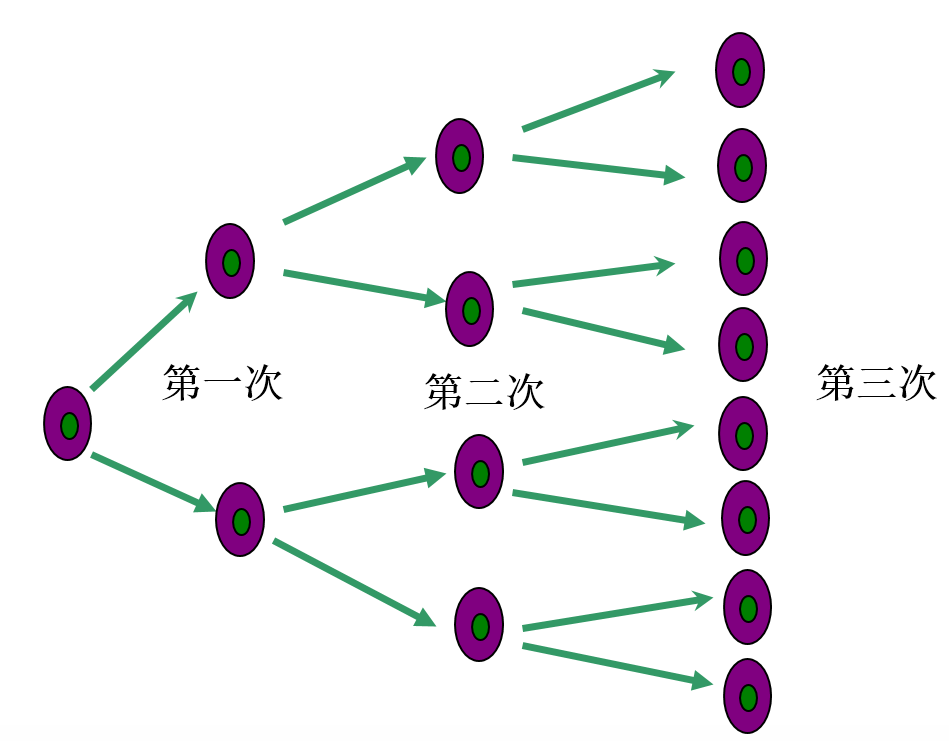
\includegraphics[width=.6\textwidth]{assets/involution.png}
    \end{figure}
\end{frame}

\begin{frame}{乘方的概念}
    \myblock{}{
        一般地,n个相同的因数$a$相乘,记作$a^n$,读作“$a$的n次幂(或$a$的n次方)”,即\\
        
        \bmc{\underbrace{
                \bm{a} \cdot \bm{a} \cdot \bm{a} \cdot \ldots \cdot \bm{a}}_{n\ times} = a^n
            }
    }   

    \begin{figure}
        \includegraphics<2>[width=.9\textwidth]{assets/14.png}
    \end{figure}
\end{frame}

\begin{frame}{乘方的概念}
    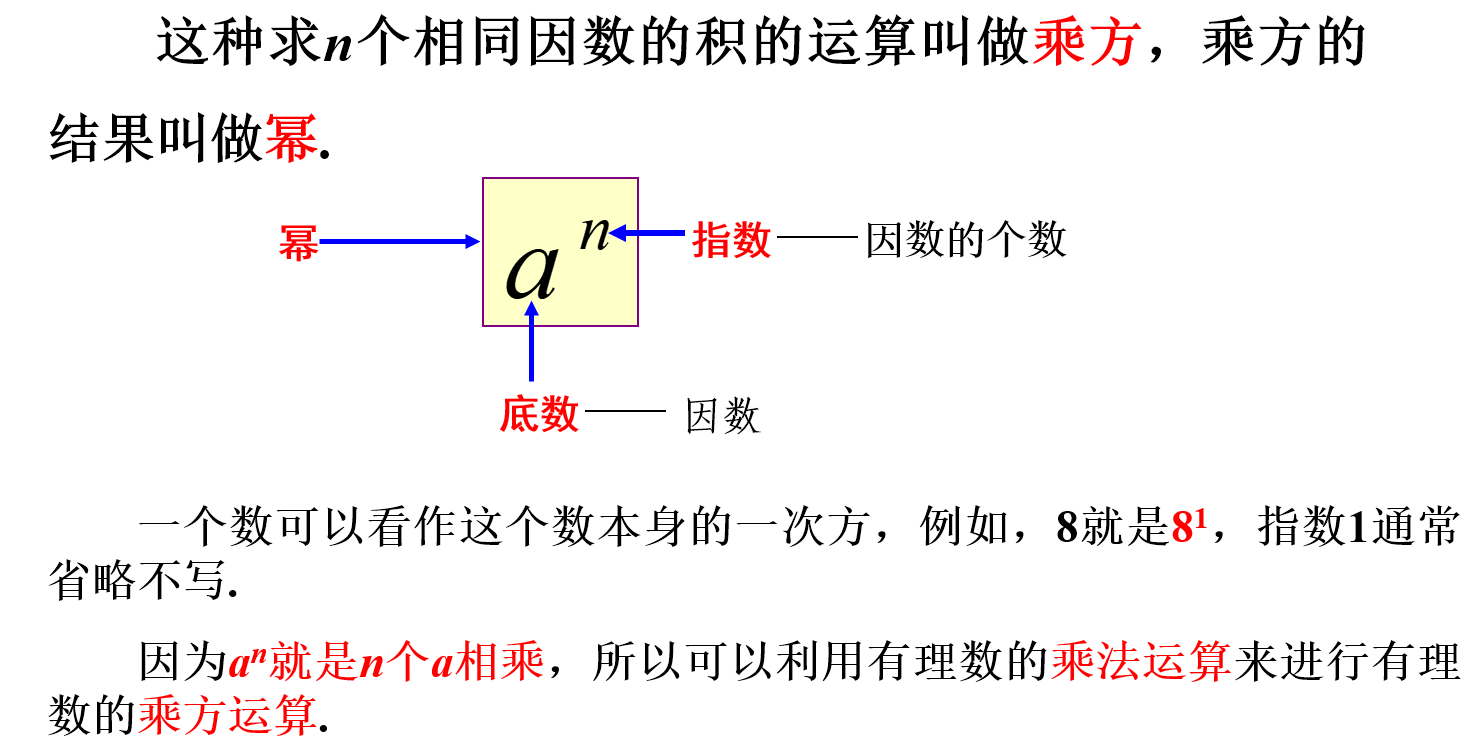
\includegraphics[width=.9\textwidth]{assets/15.png}
\end{frame}

\begin{frame}{练习1}
    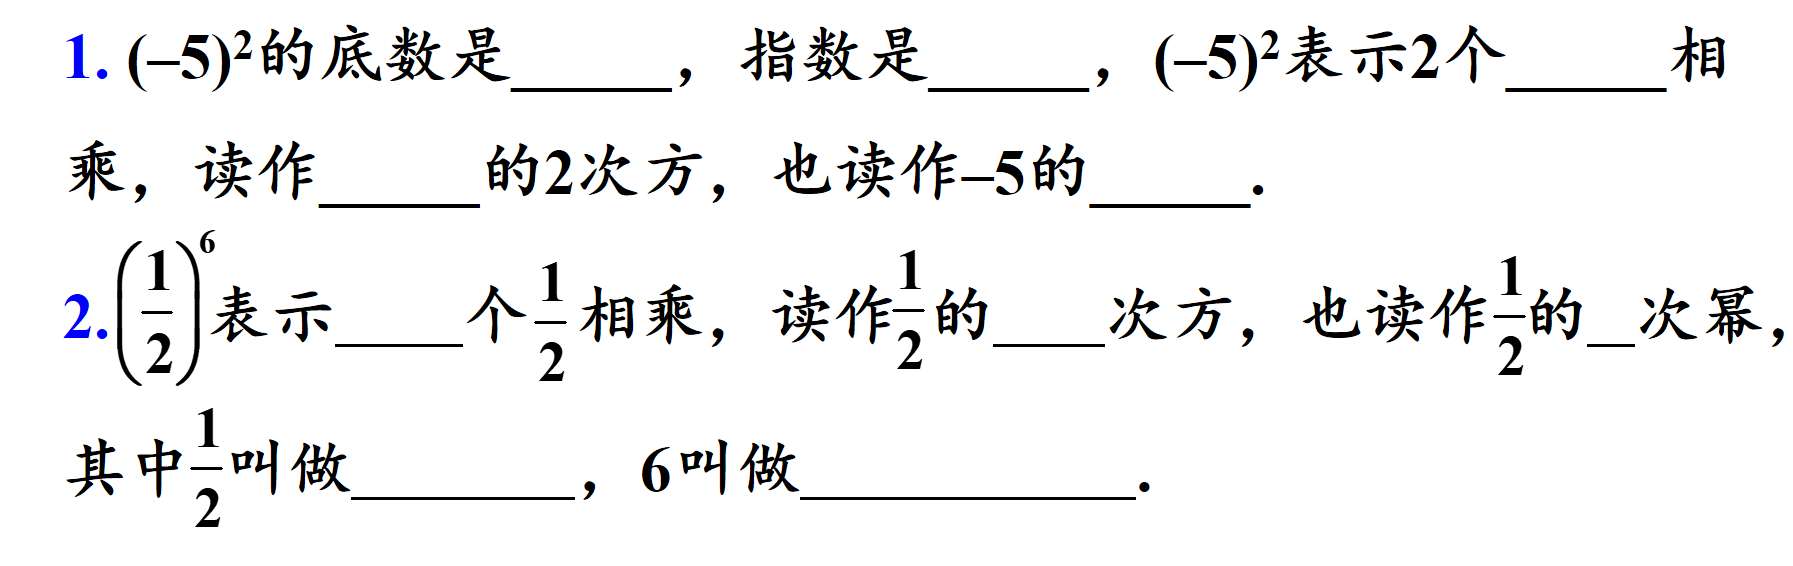
\includegraphics[width=.9\textwidth]{assets/16.png}
\end{frame}

\begin{frame}{练习2}
    \myblock{计算}{
        \bmc{(-4)^4 = }

        \vspace{1em}
        \bmc{(-\dfrac{3}{4})^3 = }

        \vspace{1em}
        若$n$为整数,求\bmc{(-1)^n}。
    }
\end{frame}

\begin{frame}{推论}
    根据有理数的乘法法则可以得出:
        \begin{itemize}
            \item 负数的\alert{奇次幂}是负数,负数的\alert{偶次幂}是正数
            \item 正数的任何正整数次幂都是正数,0的任何正整数次幂都是0
        \end{itemize}
        \only<2>{
            \makecenter{ \bmc{|x| = 8} , 方程有几个解? }}

    \myalertblock[2]{能力提升-解简单的一元二次方程}{
        \bmc{x^2 = 4}

        \bmc{x^2 = -4}

        \bmc{x^2 = 81}
    }
\end{frame}

\section{有理数的混合运算}
\begin{frame}{必备知识}
    \myblock{}{
        \begin{enumerate}
            \item 加减乘除的法则;
            \item 加法的运算律与乘法的运算律;
            \item 运算的优先级别
                \begin{itemize}
                    \item 括号(按小括号、中括号、大括号的顺序依次进行)
                    \item 乘方
                    \item 乘除
                    \item 加减
                    \item 同级运算,按从左到右的顺序进行
                \end{itemize}
        \end{enumerate}
    }
\end{frame}

\begin{frame}{练习3}
    \myblock{计算}{
        \bmc{-\dfrac{3}{4} \times [3 \times (-\dfrac{1}{3})^2 -2]}

        \vspace{1em}
        \bmc{-1^4 - \dfrac{1}{7} \times |2-(-3)^2| + (-\dfrac{1}{3}+\dfrac{3}{4}) \div (-\dfrac{1}{24})}

        \vspace{1em}
        \bmc{-0.25 \div (-\dfrac{1}{2})^2 \times (-1)^3 + (\dfrac{11}{8}+\dfrac{7}{3})\times 24}
    }
\end{frame}
\section{代数式的相关概念}

\section{一元一次方程}

\section{解方程}

\section{方程的应用与列方程}
\end{document}